% Chapter 1
\chapter{مقدمه}

در سال‌های اخیر، بیت‌کوین \cite{r1} به عنوان یکی از برجسته‌ترین ارزهای دیجیتال از زمان پیدایش آن در سال 2009 توسط ساتوشی ناکاموتو\LTRfootnote { Satoshi Nakamoto } مورد توجه قرار گرفته است. ویژگی‌های نوآورانه‌ای نظیر ناشناس بودن، کارمزد پایین تراکنش، عدم تمرکز و دسترسی دائمی به خدمات، بیت‌کوین را به موضوعی پرطرفدار در سال‌های گذشته تبدیل کرده است. با این حال، تحقیقات محدودی در زمینه تحلیل شبکه بیت‌کوین انجام شده است. تحلیل ساختار شبکه‌ تراکنش‌های بیت‌کوین از منظر شبکه‌های پیچیده بسیار مهم است زیرا می‌تواند رازهای سیستم‌های بلاکچین موجود را آشکار کند.

مهمترین مشارکت‌های این پژوهش به شرح زیر خلاصه می‌شود:

یک روش نمونه‌گیری جدید به نام پیمایش تصادفی با بازگشت برای تحلیل داده‌های تراکنش بیت‌کوین معرفی می‌گردد. روش بیان شده در حالی که پیچیدگی محاسباتی کمتری نسبت به روش های متعارف دارد، نمونه برداری\LTRfootnote { Sampling } دقیق‌تری از شبکه پیچیده بیت‌کوین ارائه می‌دهد و ویژگی‌های شبکه اصلی بیت‌کوین را حفظ می‌کند.
سپس با استفاده از روش معرفی شده، از شبکه نمونه برداری کرده و به تحلیل آن میپردازیم.
با تحلیل این شبکه پیچیده چندین مشاهده جدید از عملکرد کاربران و ساختار شبکه فعلی بیت‌کوین به دست می‌آوریم.

مشاهدات جدید درک عمیقی از ساختار شبکه بلاکچین بیت‌کوین ارائه می‌دهند و می‌توانند به بهبود امنیت و کارایی شبکه‌های بلاکچین ارزهای دیجیتال کمک کنند.
\section{مقدمه‌ای بر بلاکچین}
 
\begin{figure}[t]
\centering
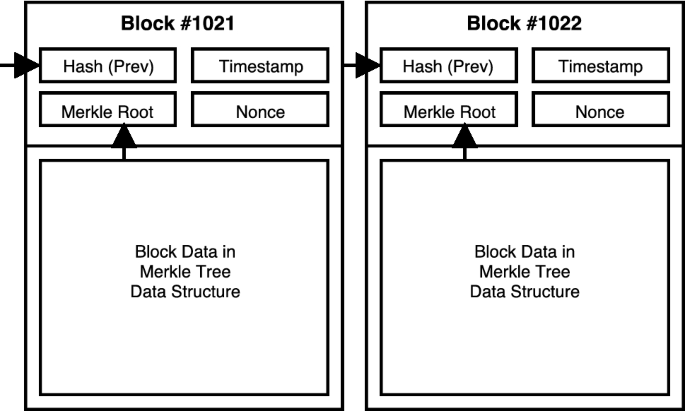
\includegraphics[height=7cm,width=10cm]{Blockchain.png}
\caption{ساختار کلی بلاکچین}
\label{bc}
\centering
\end{figure}
بلاکچین یک فناوری انقلابی است که به عنوان پایه‌ای برای بیت‌کوین و سایر ارزهای دیجیتال\LTRfootnote { Cryptocurrency } عمل می‌کند. در ساده‌ترین شکل، بلاکچین یک دفتر کل\LTRfootnote { Ledger }  توزیع شده و تغییرناپذیر است که تراکنش‌ها را به صورت امن و شفاف ذخیره می‌کند \cite{r2}.
\subsection{مفهوم بلاکچین}
همانطور که در شکل \ref{bc} قابل مشاهده است، ساختار بلاکچین شامل تعدادی بلاک می‌باشد که اطلاعات تراکنش‌ها رو درون خود جای داده اند و به کمک زنجیره‌ای به یکدیگر متصل شده اند. هر بلاک شامل اطلاعات زیر است:

\begin{itemize}
    \item \textbf{اطلاعات تراکنش‌ها:}  لیستی از تراکنش‌های انجام شده.
    \item \textbf{هش\footnote{ Hash } بلاک قبلی:} یک رشته منحصر به فرد که به بلاک قبلی اشاره می‌کند و بلاک‌ها را به یکدیگر متصل می‌سازد.
    \item \textbf{هش بلاک فعلی:} یک رشته منحصر به فرد که به محتوای بلاک اشاره دارد و با استفاده از الگوریتم‌های رمزنگاری ایجاد می‌شود.
\end{itemize}

\subsection{نحوه کار بلاکچین}

بلاکچین یک سیستم توزیع‌شده و غیرمتمرکز است که امکان ثبت و ذخیره‌سازی امن و شفاف اطلاعات را بدون نیاز به یک نهاد مرکزی فراهم می‌کند. در این بخش، نحوه کار بلاکچین را با جزئیات بیشتری بررسی می‌کنیم.

\subsubsection{تراکنش‌ها}
افراد تراکنش‌های خود را از طریق یک شبکه توزیع‌شده ارسال می‌کنند. هر تراکنش شامل اطلاعاتی نظیر فرستنده، گیرنده و مقدار ارز منتقل شده است. این تراکنش‌ها در شبکه منتشر می‌شوند تا توسط گره‌های\LTRfootnote { Node } موجود در شبکه بررسی و تایید شوند.

\subsubsection{تایید تراکنش‌ها}
تراکنش‌ها توسط گره‌های شبکه تایید می‌شوند. گره‌ها دستگاه‌هایی هستند که بلاکچین را پشتیبانی می‌کنند و مسئولیت تایید صحت تراکنش‌ها را بر عهده دارند. برای تایید تراکنش‌ها، گره‌ها از الگوریتم‌های رمزنگاری استفاده می‌کنند تا اطمینان حاصل کنند که فرستنده تراکنش واقعاً مالک ارز دیجیتال مورد نظر است.

\subsubsection{ایجاد بلاک جدید}
پس از تایید تراکنش‌ها، این تراکنش‌ها به یک بلاک جدید اضافه می‌شوند. هر بلاک شامل مجموعه‌ای از تراکنش‌های تایید شده است که به همراه یک شناسه یکتا (هش بلاک) و هش بلاک قبلی به بلاکچین اضافه می‌شود. فرآیند ایجاد بلاک جدید معمولاً توسط استخراج‌کنندگان\LTRfootnote { Miners }  انجام می‌شود که از قدرت محاسباتی خود برای حل مسائل پیچیده ریاضی استفاده می‌کنند.

\subsubsection{افزودن به زنجیره}
بلاک جدید به زنجیره بلاک‌های قبلی متصل می‌شود. این اتصال با استفاده از هش بلاک قبلی و هش بلاک جدید انجام می‌شود. هش بلاک جدید باید به گونه‌ای محاسبه شود که با معیارهای مشخصی سازگار باشد، که این امر به تضمین امنیت و یکپارچگی بلاکچین کمک می‌کند.

\subsubsection{توزیع بلاکچین}
نسخه جدید بلاکچین به تمام گره‌های شبکه ارسال می‌شود. پس از تایید و صحت سنجی بلاک، آنها نسخه‌های خود را به‌روزرسانی می‌کنند. این فرآیند به گره‌های موجود در شبکه اجازه می‌دهد تا از یک نسخه مشترک و به‌روز بلاکچین استفاده کنند. این امر باعث شفافیت شبکه و همچنین غیرمتمرکز بودن آن می‌شود.

\subsection{مزایای بلاکچین}

بلاکچین به عنوان یک فناوری نوآورانه دارای مزایا و کاربردهای فراوانی است که بهبودهای قابل توجهی در مقایسه با سیستم‌های سنتی ارائه می‌دهد. در این بخش، برخی از مهم‌ترین مزایای بلاکچین شرح داده می‌شوند.

\subsubsection{توزیع شدگی}
بلاکچین به صورت توزیع شده عمل می‌کند، به این معنا که داده‌ها در شبکه‌ای از گره‌ها ذخیره می‌شوند و هیچ نقطه متمرکزی برای حمله وجود ندارد. این ویژگی باعث افزایش مقاومت شبکه در برابر حملات سایبری و کاهش خطر از دست رفتن داده‌ها می‌شود.

\subsubsection{شفافیت}
یکی از ویژگی‌های بارز بلاکچین، شفافیت آن است. تمامی تراکنش‌ها در بلاکچین عمومی هستند و هر کسی می‌تواند آنها را مشاهده کند. این شفافیت موجب افزایش اعتماد کاربران و کاهش احتمال تقلب می‌شود.
هرچند که امروزه سیستم‌های خصوصی مبتنی بر بلاکچین نیز در حال گسترش و تولید اند.

\subsubsection{تغییرناپذیری}
تراکنش‌های ذخیره شده در بلاکچین قابل تغییر یا حذف نیستند. هر بلاک شامل هش بلاک قبلی است و این اتصال به زنجیره‌ای از بلاک‌ها منجر به تغییرناپذیری داده‌ها می‌شود. این ویژگی، از تغییرات غیرمجاز و دستکاری در داده‌ها جلوگیری می‌کند.

\subsubsection{امنیت}
بلاکچین از الگوریتم‌های رمزنگاری پیچیده برای ایجاد هش استفاده می‌کند که امنیت داده‌ها را تضمین می‌کند. هر تراکنش و بلاک توسط الگوریتم‌های رمزنگاری محافظت می‌شوند و این امر مانع از دسترسی غیرمجاز و هک شدن داده‌ها می‌شود.


\section{مقدمه‌ای بر شبکه‌های پیچیده} 
شبکه‌های پیچیده، به عنوان یک زیرشاخه مهم در علم شبکه‌ها، ساختارها و رفتارهای پیچیده‌ای را مدل‌سازی و بررسی می‌کنند. به دلیل پیچیدگی بالای موجود در اینگونه شبکه‌ها، تحلیل و مطالعه خواصشان نیازمند روش‌ها و تکنیک‌های منحصربه‌فرد می‌باشد. این شبکه‌ها معمولاً از عناصر متعدد و پیچیده‌ای مانند گره‌ها (نقاط) و پیوندها (لبه‌ها) تشکیل شده‌اند که با هم به شکل‌دهی ساختارهای غیرمنظم و پویایی منجر می‌شوند. این ساختار پیچیده با استفاده از گراف‌ها مدل می‌شود. از این رو تئوری گراف و بررسی ساختار شبکه‌های پیچیده، بسیار شباهت دارند.

شبکه‌های پیچیده در زندگی مدرن امروزی نقش مهمی ایفا می‌کنند. همچنین شاهد حضور پررنگ شبکه‌های پیچیده در زندگی روزمره انسان هستیم. یکی از این شبکه‌های پیچیده؛ شبکه تراکنش‌های بیت‌کوین، به عنوان یک رمزارز مورد استفاده توسط مردم می‌باشد.

\subsection{ویژگی‌های شبکه‌های پیچیده}
برای بررسی و آشنایی با شبکه‌های پیچیده، نیازمند شناخت ویژگی‌ها و خصوصیات اینگونه شبکه‌ها می‌باشیم.

در ادامه به بررسی اجمالی ویژگی‌های یک شبکه پیچیده می‌پردازیم.
\begin{itemize}
    \item \textbf{تعداد زیاد گره‌ها و پیوندها:} شبکه‌های پیچیده معمولاً شامل تعداد زیادی گره و پیوند هستند. به عنوان مثال، در شبکه‌های اجتماعی، گره‌ها نماینده افراد و پیوندها نماینده روابط اجتماعی بین آن‌ها هستند و یا در شبکه پیچیده بیت‌کوین، آدرس‌های تراکنش نماینده گره‌ها و تراکنش انجام شده میان آدرس مبدا و آدرس مقصد نمایانگر پیوند جهت‌دار و وزن‌دار میان دو گره می‌باشد.
    
    \item \textbf{ساختار غیرمنظم:} شبکه‌های پیچیده دارای ساختاری غیرمنظم و پیچیده هستند. این ساختار به دلیل تعداد بالای پیوندها و پویایی شبکه، به صورت مرتب و منظم نیست. به عبارت دیگر، الگوی خاصی برای چگونگی اتصال گره‌ها به یکدیگر وجود ندارد و شبکه‌ها به صورت تصادفی و پویا تغییر می‌کنند.
    
    \item \textbf{همبستگی و ساختارهای سلسله‌مراتبی:} شبکه‌های پیچیده ممکن است دارای همبستگی‌ها و ساختارهای سلسله‌مراتبی باشند. این به این معناست که برخی از گره‌ها به عنوان گره‌های اصلی یا مرکزی عمل می‌کنند و بسیاری از گره‌های دیگر به این گره‌های مرکزی متصل می‌شوند.
\end{itemize}

\pagebreak

~\section{ساختار شبکه بیت‌کوین\footnote{ Bitcoin Network Construction }}
\begin{figure}[t]
\centering
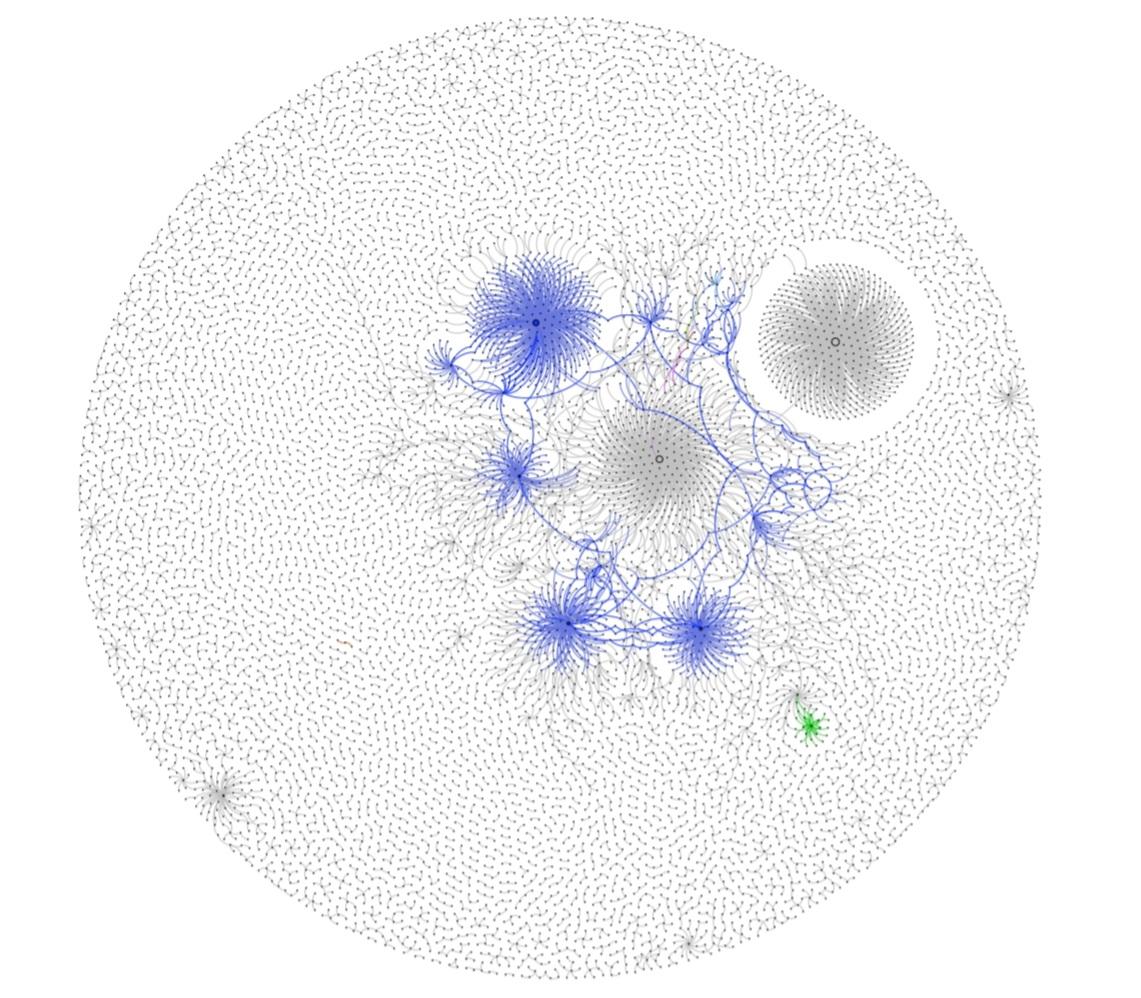
\includegraphics[height=6cm,width=7.5cm]{BTC_VISUAL.jpg}
\caption{نمایی از شبکه تراکنش بیت‌کوین با 10,000 گره منتخب \cite{r0}}
\label{btcv}
\centering
\end{figure}
این مقاله به بررسی تراکنش‌های بیت‌کوین پرداخته است که در آن، هر تراکنش می‌تواند چندین آدرس ورودی و چندین آدرس خروجی داشته باشد. به عنوان مثال، یک تراکنش از $x$ آدرس ورودی و $y$ آدرس خروجی استخراج می‌شود و به صورت $x \times y$ نمایش داده می‌شود. سپس، هر گره نماینده یک آدرس بیت‌کوین خواهد بود، همچنین هر لبه جهت‌دار نشان‌دهنده جهت انجام آن تراکنش است و وزن لبه متناسب با ارزش تراکنش مشخص می‌شود.

مقاله یک شبکه تراکنش بیت‌کوین را به یک گراف جهت‌دار وزنی تبدیل می‌کند که با \mbox{$G = (V, E, W)$} نشان داده می‌شود، جایی که $V$ مجموعه گره‌ها، $E$ مجموعه لبه‌ها و $W$ مجموعه وزن‌ها است. هر لبه به صورت $e_{ij} = (i, j, w_{ij})$ نمایش داده می‌شود. مجموعه $E$ با $N$ گره می‌تواند به صورت یک ماتریس $N \times N$ نمایش داده شود که اساساً یک ماتریس مجاورت است و با $A$ نشان داده می‌شود. برای هر عنصر $a_{ij}$ در $A$، داریم:

\[
a_{ij} = 
\begin{cases} 
w_{ij} & \text{ تعریف شده باشد} e_{ij} \text{اگر }  \\ 
0 & \text{در غیر این صورت} 
\end{cases}
\]
\newpage
داده‌های مورد استفاده در این مقاله؛ از تراکنش‌ها و آدرس تراکنش‌های موجود در پایگاه داده پروژه بیت‌کوین، از ژانویه 2017 تا ژانویه 2018 بدست آمده اند که شامل بیش از 148,000,000 گره و 870,000,000 لبه می‌باشند. شکل \ref{btcv} نمایی از شبکه تراکنش بیت‌کوین با 10,000 گره منتخب را نشان می‌دهد.

\section{نمونه‌برداری از شبکه بیت‌کوین}

شبکه تراکنش بیت‌کوین یک گراف بسیار بزرگ با میلیون‌ها گره است، بنابراین لازم است که یک شبکه نمونه، نماینده، برای ساده‌سازی تحلیل‌ها بدست آوریم. برخی از مطالعات قبلی نشان داده‌اند که روش‌های نمونه‌برداری مبتنی بر پیاده‌روی تصادفی\footnote{ Random walk(RW)} می‌توانند خواص ساختاری شبکه بلاکچین مقیاس آزاد\footnote{Scale-free} را به خوبی حفظ کنند. بنابراین، در این مقاله نیز یک روش نمونه‌برداری گراف، مبتنی بر پیاده‌روی تصادفی، برای نمایندگی شبکه بلاکچین بیت‌کوین طراحی معرفی می‌گردد.

\subsection{روش نمونه برداری RWFB}
در روش‌های سنتی پیاده‌روی تصادفی، گره بعدی $j$ به صورت تصادفی از همسایگان گره فعلی $i$ انتخاب می‌شود. با این حال، این روش‌ها نمی‌توانند به دقت شبکه بیت‌کوین را نمونه‌برداری کنند. برای رفع این مشکل، روش ابداعی با نام پیاده روی تصادفی با بازگشت به عقب طراحی و معرفی می‌گردد.

به طور خاص، پیاده روی تصادفی با بازگشت به عقب هنگام نمونه‌برداری از شبکه، احتمال بازگشت به گره فعلی را نیز در نظر می‌گیرد. در هر گام از پیاده‌روی تصادفی جهت‌دار، RWFB با احتمال بازگشت $p$ به گره فعلی یعنی $i$ بازمی‌گردد؛ و با احتمال $1 - p$ یک همسایه تصادفی از میان $k_i$ همسایه‌های خود را انتخاب می‌کند، بنابراین هر کدام دارای احتمالی برابر با $(1 - p) / k_i$ هستند. احتمال RWFB را که با $P_{RWFB_i}$ نشان داده می‌شود، به صورت زیر تعریف می‌کنیم:
\[
P_{RWFB_i} = 
\begin{cases} 
p & \text{بازگشت به گره $i$} \\
\frac{1 - p}{k_i} & \text{انتقال به همسایه $j$ از گره $i$ }
\end{cases}
\]
\\
پیاده‌روی همیشه از یک گره تصادفی شروع می‌شود. علاوه بر این، اگر در طول پیاده‌روی به بن‌بست برخورد کند، یک گره تصادفی دیگر برای ادامه انتخاب می‌شود تا زمانی که اندازه نمونه‌برداری به مقدار دلخواه و موردنیازمان برسد.



حال پس از اتمام نمونه‌برداری نیاز به تعریف گراف جدید داریم. گراف نمونه‌برداری شده با تابع بازگشت را به عنوان $G_{RWFB} = (V_i, E_{i,j}, w_{i,j})$ دوباره تعریف می‌کنیم. در این گراف جهت‌دار و وزن‌دار، گره‌ها همان رئوس پیموده شده هستند و لبه‌ها همان گام‌هایی اند که پیموده ایم.


\subsection{ارزیابی روش نمونه‌برداری RWFB}
جدول ~\ref{eval}، مقایسه روش‌های نمونه‌برداری با استفاده از آماره D-statistic K-S را نشان می‌دهد.
این آماره مشخص می‌کند که ورودی هایش در معیارهای مختلف چه‌قدر متفاوت اند. هرچه تفاوت دو ورودی اش، که گراف نیز می‌باشند، بیشتر باشد عدد حاصل به یک نزدیکتر است.
هرچه عدد حاصل به صفر نزدیکتر باشد یعنی تفاوت میان گراف نمونه\footnote{$G_{RWFB} = (V_i, E_{i,j}, w_{i,j})$} و گراف اصلی\footnote{$G = (V, E, W)$} کمتر بوده است.

مطابق با جدول ~\ref{eval} می‌توان نتیجه گرفت؛ روش ابداعی عملکرد بهتری را نسبت به سایر روش‌های سنتی داشته است، گراف اصلی را بهتر نمونه‌برداری کرده و دارای خواص نسبتا مشابه با آن می‌باشد.
\begin{table}[t]
\centering
\begin{LTR}
\begin{latin}
\begin{tabular}{cccccc}
\hline
\textbf{Sampling Method} & \textbf{Degree} & \textbf{Clustering} & \textbf{Betweenness} & \textbf{Closeness} & \textbf{Average} \\
\hline
\textbf{RWFB} & 0.120 & 0.045 & 0.091 & 0.429 & \textbf{0.171} \\
RWS & 0.293 & 0.046 & 0.536 & 0.618 & 0.373 \\
RN & 0.895 & 0.053 & 0.151 & 0.433 & 0.383 \\
RE & 0.275 & 1.000 & 0.067 & 0.549 & 0.473 \\
FF & 0.187 & 1.000 & 0.075 & 0.669 & 0.483 \\
SB & 0.409 & 0.025 & 0.583 & 0.645 & 0.415 \\
\hline
\end{tabular}
\end{latin}
\end{LTR}
\caption{مقایسه روش‌های نمونه‌برداری با استفاده از  D-statistic K-S}
\label{eval}
\end{table}


